$l$ and $m$ are two parallel lines intersected by another pair of parallel lines $p$ and $q (\figref{fig:9.7.1.4})$,show that $\triangle ABC \cong \triangle CDA$.

\textbf{Figure :}
\begin{figure}[H]
    \centering
	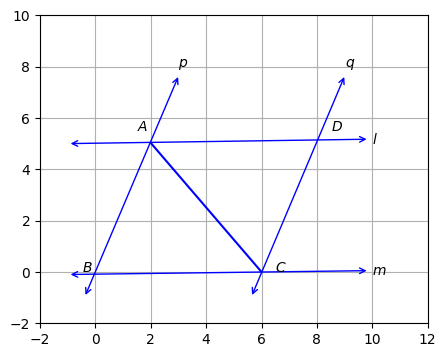
\includegraphics[width=0.75\columnwidth]{chapters/9/7/1/4/fig/em1.png}
    \caption{Required parallelogram}
    \label{fig:9.7.1.4}
\end{figure}

\textbf{Solution :}
\begin{table}[H]
    \centering
        \begin{tabular}{|c|c|c|}
    \hline
    \textbf{Input Parameters} &\textbf{Description} &\textbf{Value} \\
    \hline
     $\vec{O}$& Center(at origin)&$\vec{0}$\\
     \hline
 $r$ & Radius &1\\
 \hline
 $\theta$&$\angle PQR$&$100\degree$\\
 \hline
 $\theta_1$&$\angle NOQ $&$\theta_1\degree$\\
 \hline
 $\theta_2$&$\angle NOP $&$165\degree$\\
 \hline
 $\theta_3$&$\angle NOR $&$5\degree$\\
 \hline
  \end{tabular}

    \caption{Table of input parameters}
    \label{tab:9.7.1.4.1}
\end{table}

\begin{table}[H]
    \centering
    \begin{tabular}{|c|c|c|}
    \hline
        \textbf{Output Parameters} &\textbf{Description} &\textbf{Value} \\
\hline
          $\vec{P}$ & Point &$\myvec{\cos{\theta_1}\\\sin{\theta_1}}$ \\

         \hline
          $\vec{Q}$ & Point &$\myvec{\cos{\theta_2}\\\sin{\theta_2}}$ \\
         \hline
          $\vec{R}$ & Point &$\myvec{\cos{\theta_3}\\\sin{\theta_3}}$ \\
         \hline
          $\vec{S}$ & Point &$\myvec{\cos{\theta_4}\\\sin{\theta_4}}$ \\
         \hline
    \end{tabular}


    \caption{Table of output parameters}
    \label{tab:9.7.1.4.2}
\end{table}  
So,$\triangle ABC \cong \triangle CDA.\brak{by A-A-S}\brak{proved}$
